\documentclass[crop,tikz]{standalone}
\def\pixels{
  {0,1,0},
  {1,2,1},
  {0,1,0},
}
\definecolor{pixel 0}{HTML}{FFFFFF}
\definecolor{pixel 1}{HTML}{C0C0C0}
\definecolor{pixel 2}{HTML}{000000}
\begin{document}
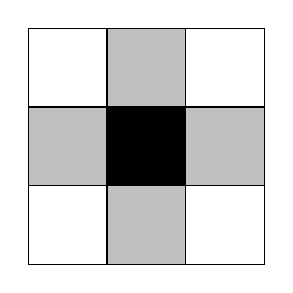
\begin{tikzpicture}
  \foreach \line [count=\y] in \pixels {
    \foreach \pix [count=\x] in \line {
      \draw[fill=pixel \pix] (\x,-\y) rectangle +(1,1);
    }
  }
\end{tikzpicture}
\end{document}